%%% Copyright (C) 2020 Vincent Goulet
%%%
%%% Ce fichier fait partie du projet
%%% «Rédaction avec LaTeX»
%%% https://gitlab.com/vigou3/formation-latex-ul
%%%
%%% Cette création est mise à disposition sous licence
%%% Attribution-Partage dans les mêmes conditions 4.0
%%% International de Creative Commons.
%%% https://creativecommons.org/licenses/by-sa/4.0/

\section{Présentation de {\TeX} et {\LaTeX}}

\begin{frame}
  \frametitle{Ce que c'est}
  \begin{columns}
    \begin{column}{.5\textwidth}
      \begin{itemize}
      \item {\TeX} est un système de mise en page (\emph{typesetting})
        ou de préparation de documents
      \item {\LaTeX} est un ensemble de macro-commandes pour faciliter
        l'utilisation de {\TeX}
      \item Langage de balisage (\emph{Markup Language}) pour indiquer
        la mise en forme du texte
      \item Accent mis sur la production de documents de grande
        qualité à la typographie soignée (surtout pour les
        mathématiques)
      \end{itemize}
    \end{column}
    \begin{column}{.5\textwidth}
      \centering
      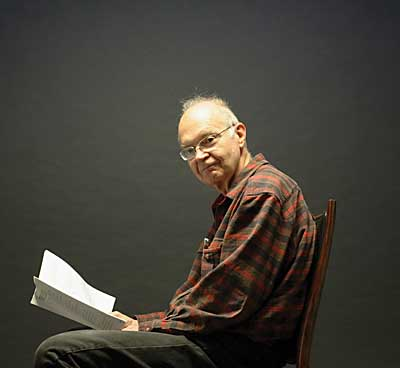
\includegraphics[width=\linewidth]{images/knuth} \\
      \footnotesize Donald Knuth, créateur de \TeX
    \end{column}
  \end{columns}
\end{frame}

\begin{frame}
  \frametitle{Ce que ce n'est pas}
  \begin{tabular}{lcl}
    Un traitement de texte & \faArrowRight & priorité accordée
                                             à la qualité de
                                             la mise en page \\[6pt]
    WYSIWYG & \faArrowRight & plutôt What You See Is What
                              You \emph{Mean} \\[6pt]
    Incompatible & \faArrowRight & format identique sur tous
                                   les systèmes d'exploitation \\[6pt]
    Instable & \faArrowRight & noyau arrivé à maturité \\[6pt]
    Imprévisible & \faArrowRight & {\LaTeX} fait ce qu'on
                                   lui demande, ni plus, ni moins
  \end{tabular}
\end{frame}

\begin{frame}
  \frametitle{Quelques choses simples à réaliser avec {\LaTeX}}

  \begin{itemize}
  \item Page de titre
  \item Table des matières
  \item Numérotation des pages
  \item Figures et tableaux: disposition, numérotation, renvois
  \item Équations mathématiques: disposition, numérotation, renvois
  \item Citations et composition de la bibliographie
  \item Coupure de mots
  \item Document recto verso
  \end{itemize}
\end{frame}

\begin{frame}[fragile=singleslide]
  \frametitle{Faits amusants}
  \begin{itemize}
  \item {\TeX} est aujourd'hui considéré exempt de bogue
  \item Récompense si vous en trouvez un!
  \item Numéro de version de {\TeX} converge vers $\pi$:
\begin{lstlisting}
$ tex --version
TeX `\textbf{3.14159265}' (TeX Live 2020)
kpathsea version 6.3.2
Copyright 2020 D.E. Knuth.
[...]
\end{lstlisting} %$
  \end{itemize}
\end{frame}

\begin{frame}
  \frametitle{Processus de création d'un document {\LaTeX}}
  \Huge
  \begin{minipage}[t]{0.25\textwidth}
    \centering
    \faFile*[regular] \\ \bigskip
    \small
    rédaction du texte et balisage avec un \alert{éditeur de texte}
  \end{minipage}
  \hfill\faArrowRight\hfill
  \begin{minipage}[t]{0.25\textwidth}
    \centering
    \faCogs \\  \bigskip
    \small
    compilation avec un \alert{moteur} {\TeX} depuis la ligne de commande
  \end{minipage}
  \hfill\faArrowRight\hfill
  \begin{minipage}[t]{0.3\textwidth}
    \centering
    \faFilePdf[regular] \\  \bigskip
    \small
    visualisation avec une visionneuse PDF (Aperçu,
    SumatraPDF, etc.)
  \end{minipage}
\end{frame}

\begin{exercice}
  Démarrer le logiciel \alert{Texmaker} (Windows), \alert{TeXShop}
  (macOS) ou tout autre éditeur ou logiciel intégré de rédaction de
  votre choix.

  \begin{enumerate}
  \item Ouvrir et compiler le fichier \fichier{exercice\_minimal.tex}.
  \item Ajouter du texte en français (avec accents) et observer le
    résultat.
  \end{enumerate}
\end{exercice}

\begin{exercice}
  Question de voir ce que {\LaTeX} peut faire, compiler le document
  élaboré \fichier{exercice\_demo.tex} de la manière suivante:
  \begin{enumerate}[i)]
  \item une fois avec \code{LaTeX};
  \item une fois avec \code{BibTeX};
  \item deux à trois fois avec \code{LaTeX}.
  \end{enumerate}
\end{exercice}

%%% Local Variables:
%%% TeX-master: "formation-latex-ul-diapos"
%%% TeX-engine: xetex
%%% coding: utf-8
%%% End:
